\documentclass[a4paper,10pt]{article}
\usepackage[utf8]{inputenc}
\usepackage[table,xcdraw]{xcolor}
\usepackage{float}
\usepackage{graphicx}

\begin{document}

\section*{Número de linhas}

\begin{table}[!h]
\begin{tabular}{lc}
\rowcolor[HTML]{CBCEFB} 
Função & \multicolumn{1}{l}{\cellcolor[HTML]{CBCEFB}Nº de Linhas Executáveis} \\
mat\_mult\_arm.s & 26 \\
\rowcolor[HTML]{C0C0C0} 
mat\_mult\_thumb.s & 40 \\
mat\_mult\_c.c & 5 \\
\rowcolor[HTML]{C0C0C0} 
mem\_access\_arm.s & 16 \\
mem\_access\_thumb.s & 16 \\
\rowcolor[HTML]{C0C0C0} 
mem\_access\_c\_.c & 4
\end{tabular}
\end{table}

Não contabilizado overheads como chamada de função Thumb e push/pop iniciais e finais.

\section*{Tamanho do executável}

\subsection*{Multiplicação de Matriz}
\begin{table}[H]
\begin{tabular}{ll}
\rowcolor[HTML]{CBCEFB} 
Nome do executável & Tamanho (bits) \\
mat\_arm\_O0 & 9888 \\
\rowcolor[HTML]{C0C0C0} 
mat\_arm\_O1 & 9888 \\
mat\_arm\_O2 & 9904 \\
\rowcolor[HTML]{C0C0C0} 
mat\_arm\_O3 & 9904 \\
mat\_arm\_Os & 9904 \\
\rowcolor[HTML]{C0C0C0} 
mat\_mult\_c\_arm\_O0 & 8592 \\
mat\_mult\_c\_arm\_O1 & 8592 \\
\rowcolor[HTML]{C0C0C0} 
mat\_mult\_c\_arm\_O2 & 8608 \\
mat\_mult\_c\_arm\_O3 & 8608 \\
\rowcolor[HTML]{C0C0C0} 
mat\_mult\_c\_arm\_Os & 8656 \\
mat\_mult\_c\_thumb\_O0 & 8596 \\
\rowcolor[HTML]{C0C0C0} 
mat\_mult\_c\_thumb\_O1 & 8596 \\
mat\_mult\_c\_thumb\_O2 & 8612 \\
\rowcolor[HTML]{C0C0C0} 
mat\_mult\_c\_thumb\_O3 & 8612 \\
mat\_mult\_c\_thumb\_Os & 8660 \\
\rowcolor[HTML]{C0C0C0} 
mat\_thumb\_O0 & 9888 \\
mat\_thumb\_O1 & 9888 \\
\rowcolor[HTML]{C0C0C0} 
mat\_thumb\_O2 & 9904 \\
mat\_thumb\_O3 & 9904 \\
\rowcolor[HTML]{C0C0C0} 
mat\_thumb\_Os & 9904
\end{tabular}


\end{table}

\subsection*{Acesso de Memória}

\begin{table}[H]
\begin{tabular}{ll}
\rowcolor[HTML]{CBCEFB} 
Nome do executável & Tamanho (bits) \\
mem\_access\_arm\_O0 & 9076 \\
\rowcolor[HTML]{C0C0C0} 
mem\_access\_arm\_O1 & 9076 \\
mem\_access\_arm\_O2 & 9092 \\
\rowcolor[HTML]{C0C0C0} 
mem\_access\_arm\_O3 & 9092 \\
mem\_access\_arm\_Os & 9092 \\
\rowcolor[HTML]{C0C0C0} 
mem\_access\_c\_arm\_O0 & 8596 \\
mem\_access\_c\_arm\_O1 & 8596 \\
\rowcolor[HTML]{C0C0C0} 
mem\_access\_c\_arm\_O2 & 8612 \\
mem\_access\_c\_arm\_O3 & 8612 \\
\rowcolor[HTML]{C0C0C0} 
mem\_access\_c\_arm\_Os & 8660 \\
mem\_access\_c\_thumb\_O0 & 8600 \\
\rowcolor[HTML]{C0C0C0} 
mem\_access\_c\_thumb\_O1 & 8600 \\
mem\_access\_c\_thumb\_O2 & 8616 \\
\rowcolor[HTML]{C0C0C0} 
mem\_access\_c\_thumb\_O3 & 8616 \\
mem\_access\_c\_thumb\_Os & 8664 \\
\rowcolor[HTML]{C0C0C0} 
mem\_access\_thumb\_O0 & 9116 \\
mem\_access\_thumb\_O1 & 9116 \\
\rowcolor[HTML]{C0C0C0} 
mem\_access\_thumb\_O2 & 9132 \\
mem\_access\_thumb\_O3 & 9132 \\
\rowcolor[HTML]{C0C0C0} 
mem\_access\_thumb\_Os & 9132
\end{tabular}
\end{table}

\section*{Tempos de execução}

Foram medidos apenas o tempo de execução dos programas compilados com otimização padrão (O0).

\subsection*{Raw}

\subsubsection*{Multiplicação de Matriz}
\begin{figure}[H]
 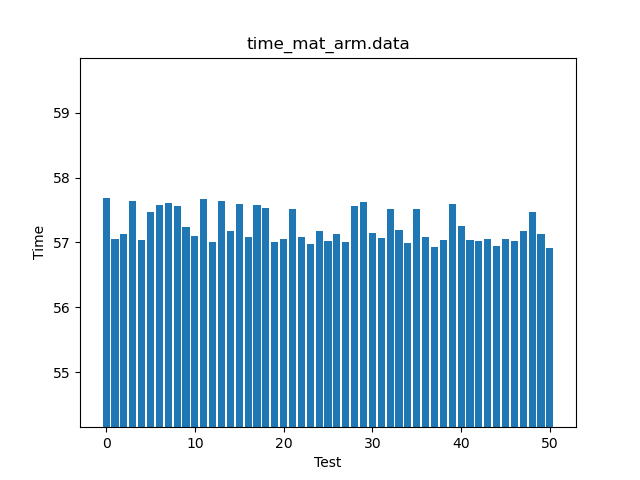
\includegraphics[width=\linewidth]{data/time_mat_arm.png}
\end{figure}

\begin{figure}[H]
 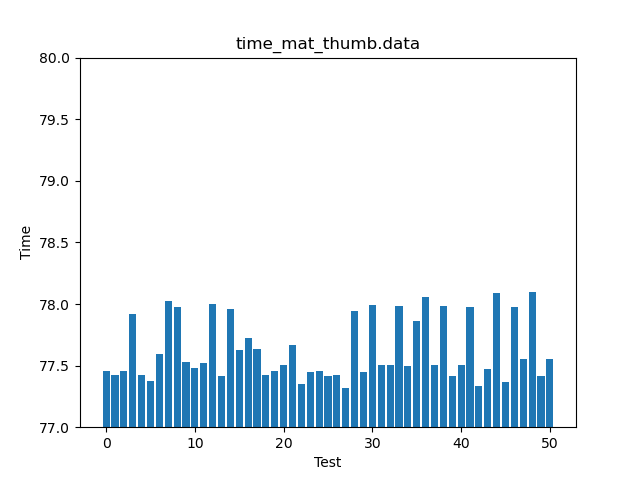
\includegraphics[width=\linewidth]{data/time_mat_thumb.png}
\end{figure}

\begin{figure}[H]
 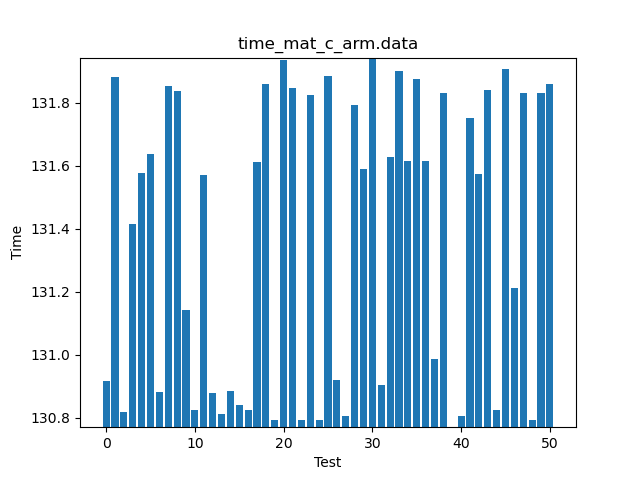
\includegraphics[width=\linewidth]{data/time_mat_c_arm.png}
\end{figure}

\begin{figure}[H]
 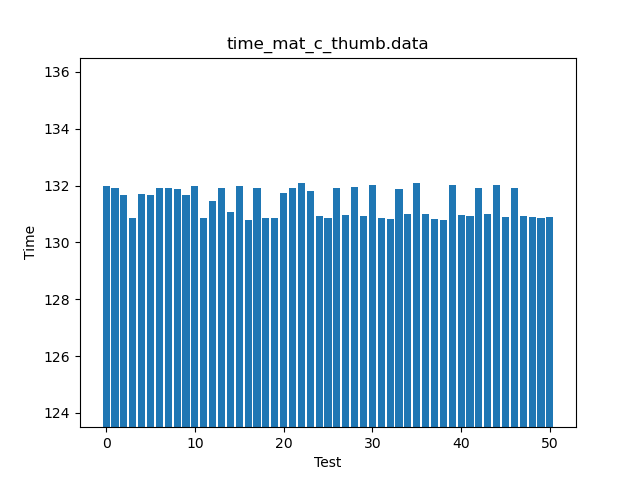
\includegraphics[width=\linewidth]{data/time_mat_c_thumb.png}
\end{figure}


\subsubsection*{Acesso de Memória}

\begin{figure}[H]
 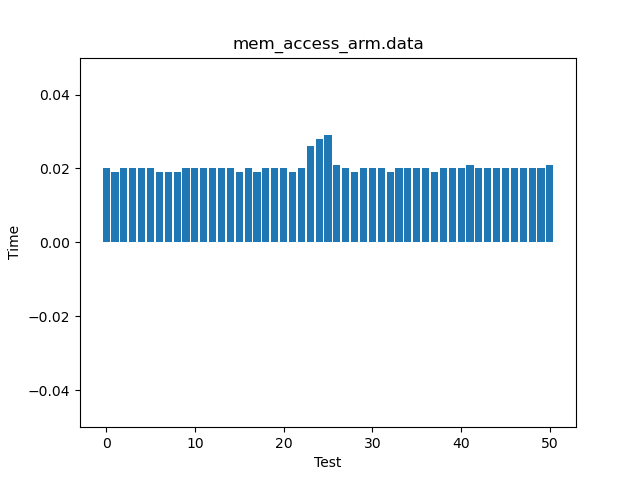
\includegraphics[width=\linewidth]{data/mem_access_arm.png}
\end{figure}

\begin{figure}[H]
 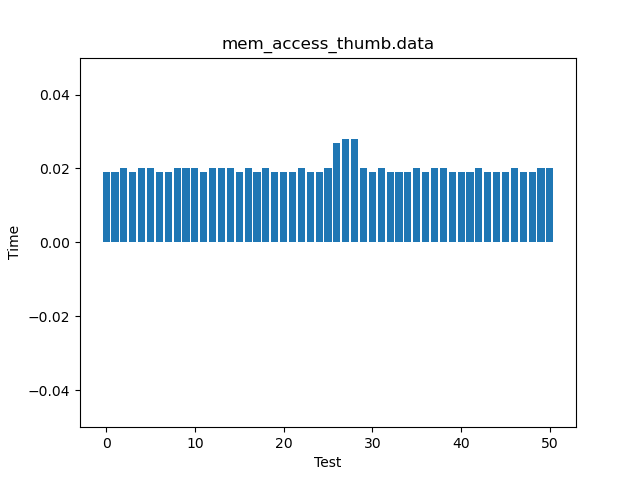
\includegraphics[width=\linewidth]{data/mem_access_thumb.png}
\end{figure}

\begin{figure}[H]
 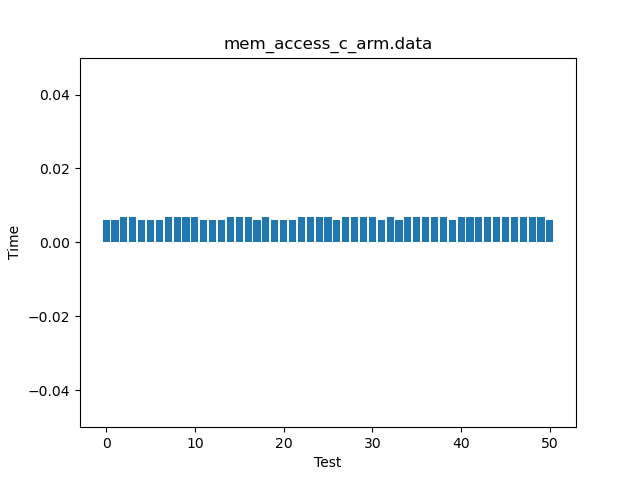
\includegraphics[width=\linewidth]{data/mem_access_c_arm.png}
\end{figure}

\begin{figure}[H]
 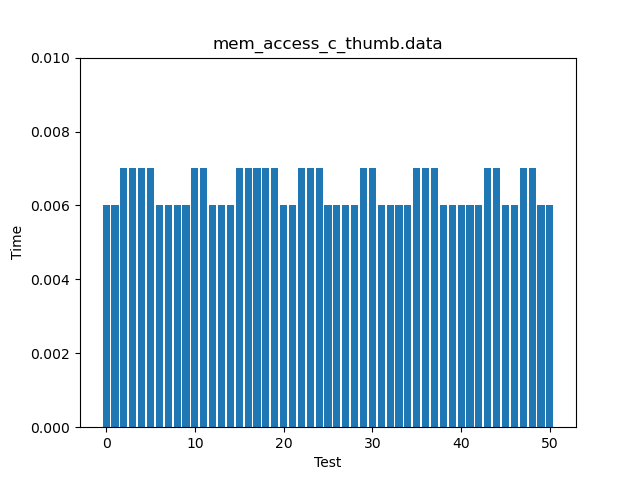
\includegraphics[width=\linewidth]{data/mem_access_c_thumb.png}
\end{figure}


\subsection*{Ordenado}

\subsubsection*{Multiplicação de Matriz}
\begin{figure}[H]
 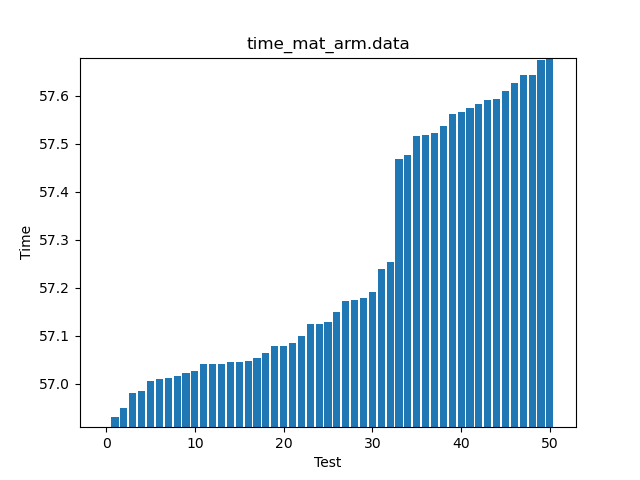
\includegraphics[width=\linewidth]{data/time_mat_arm_sorted.png}
\end{figure}

\begin{figure}[H]
 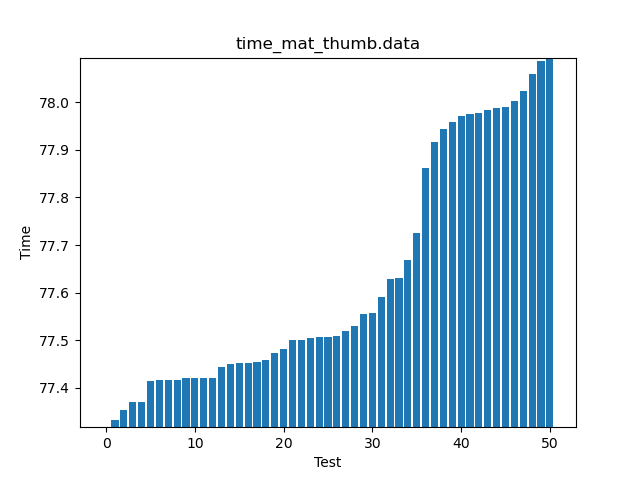
\includegraphics[width=\linewidth]{data/time_mat_thumb_sorted.png}
\end{figure}

\begin{figure}[H]
 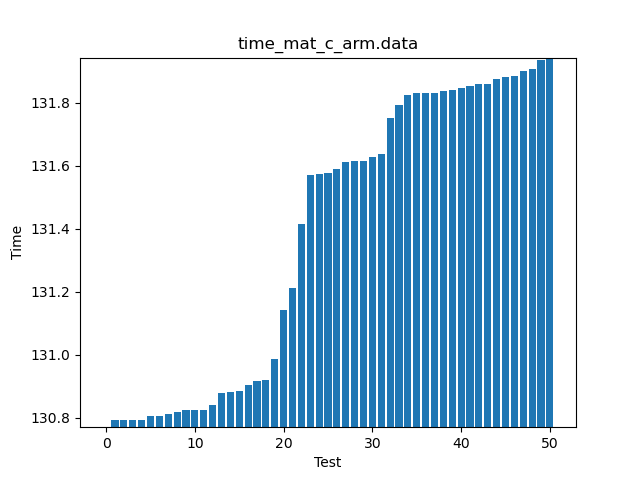
\includegraphics[width=\linewidth]{data/time_mat_c_arm_sorted.png}
\end{figure}

\begin{figure}[H]
 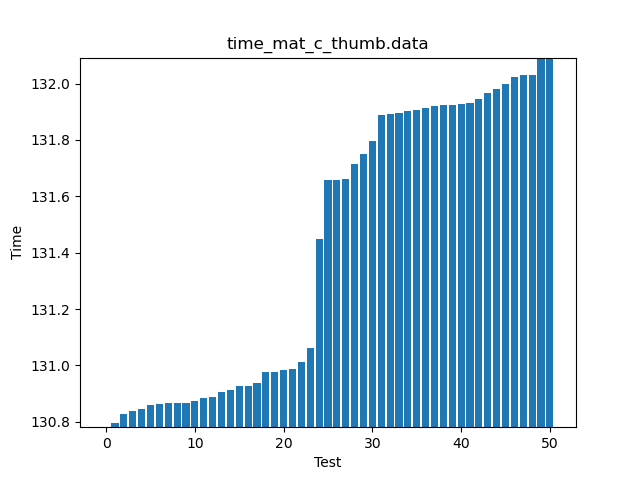
\includegraphics[width=\linewidth]{data/time_mat_c_thumb_sorted.png}
\end{figure}

\subsubsection*{Acesso de Memória}

\begin{figure}[H]
 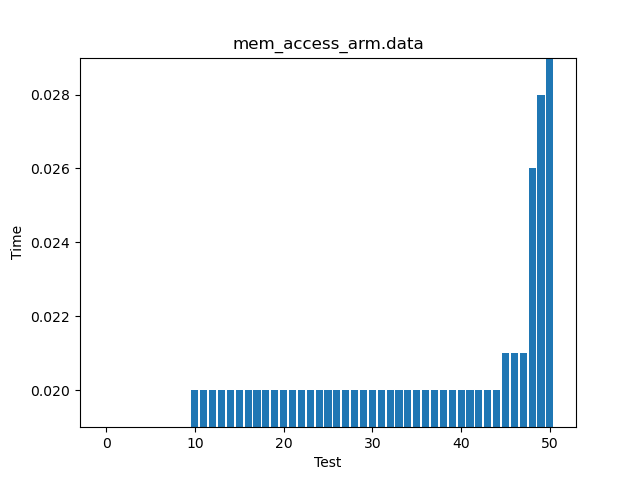
\includegraphics[width=\linewidth]{data/mem_access_arm_sorted.png}
\end{figure}

\begin{figure}[H]
 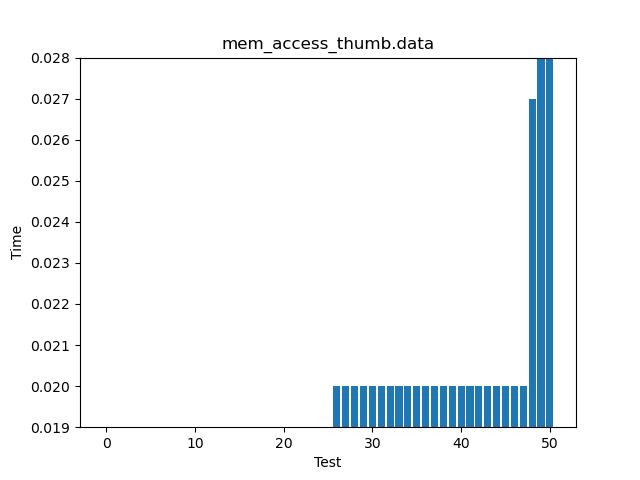
\includegraphics[width=\linewidth]{data/mem_access_thumb_sorted.png}
\end{figure}

\begin{figure}[H]
 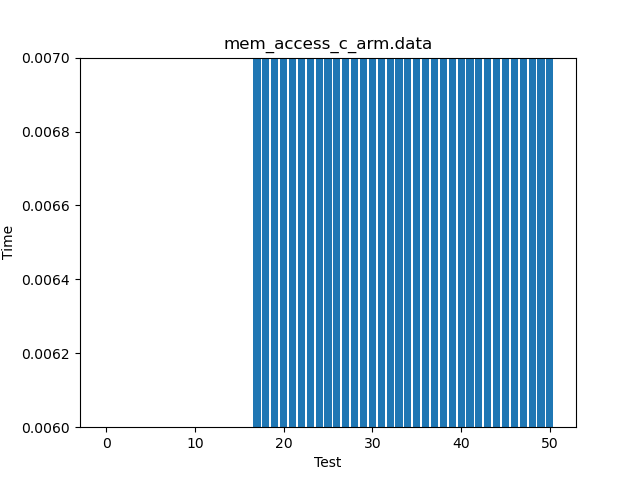
\includegraphics[width=\linewidth]{data/mem_access_c_arm_sorted.png}
\end{figure}

\begin{figure}[H]
 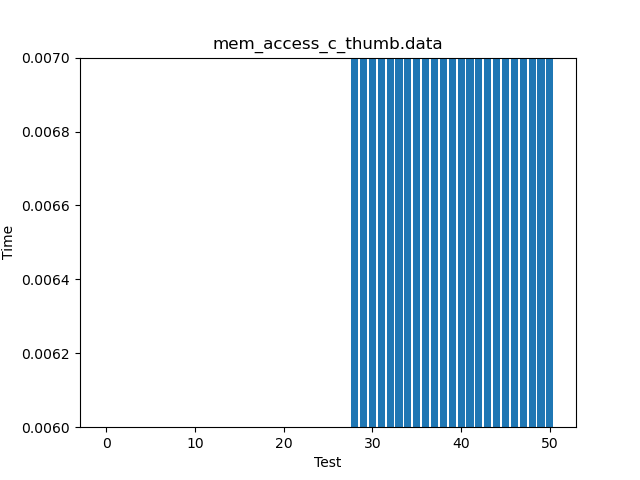
\includegraphics[width=\linewidth]{data/mem_access_c_thumb_sorted.png}
\end{figure}

\subsection*{Histogramas}
\subsubsection*{Multiplicação de Matriz}
\begin{figure}[H]
 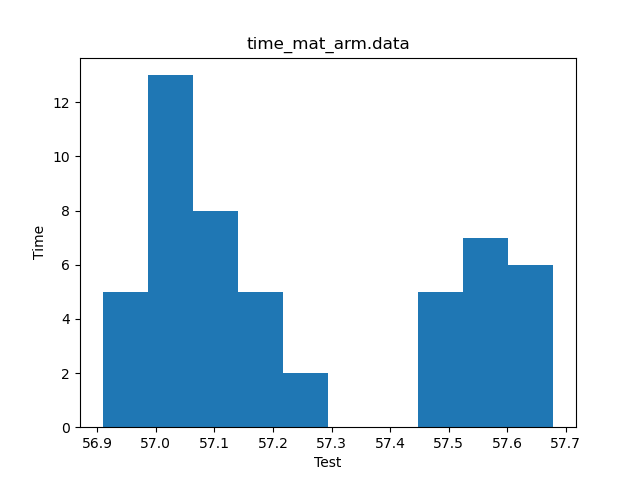
\includegraphics[width=\linewidth]{data/time_mat_arm_histogram.png}
\end{figure}

\begin{figure}[H]
 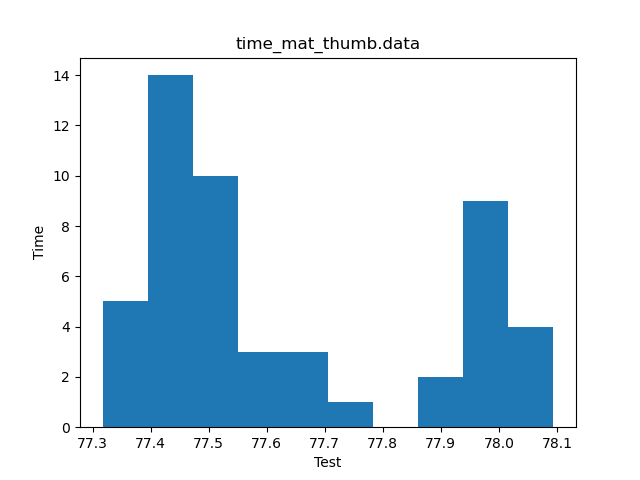
\includegraphics[width=\linewidth]{data/time_mat_thumb_histogram.png}
\end{figure}

\begin{figure}[H]
 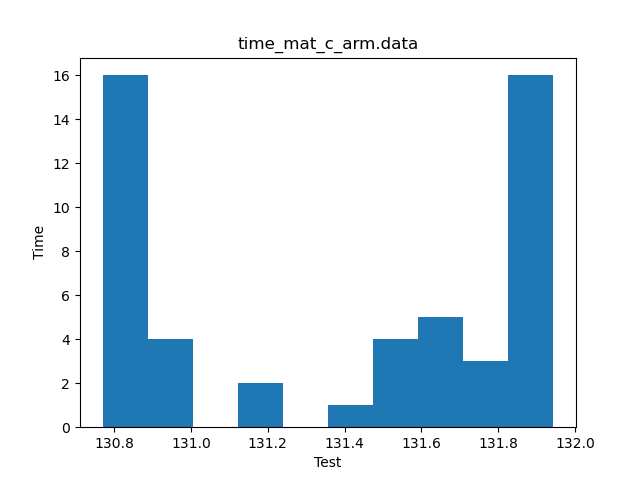
\includegraphics[width=\linewidth]{data/time_mat_c_arm_histogram.png}
\end{figure}

\begin{figure}[H]
 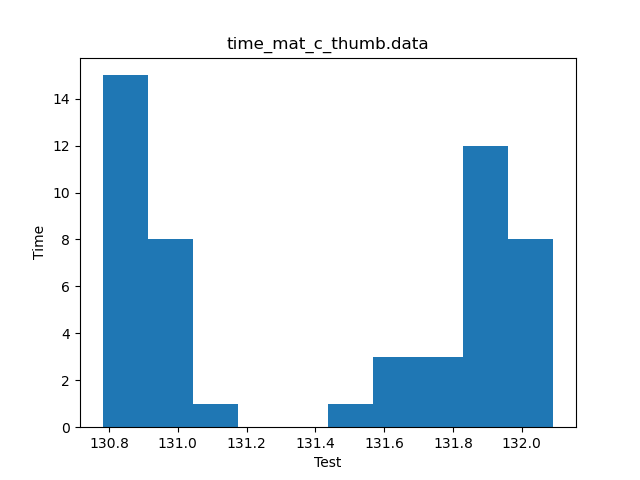
\includegraphics[width=\linewidth]{data/time_mat_c_thumb_histogram.png}
\end{figure}

\subsubsection*{Acesso de Memória}

\begin{figure}[H]
 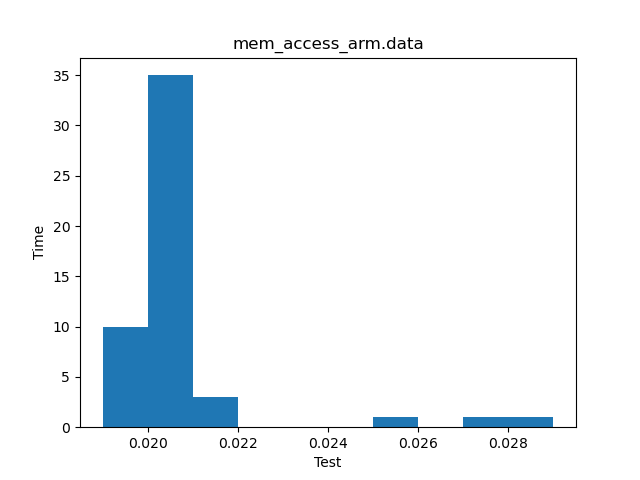
\includegraphics[width=\linewidth]{data/mem_access_arm_histogram.png}
\end{figure}

\begin{figure}[H]
 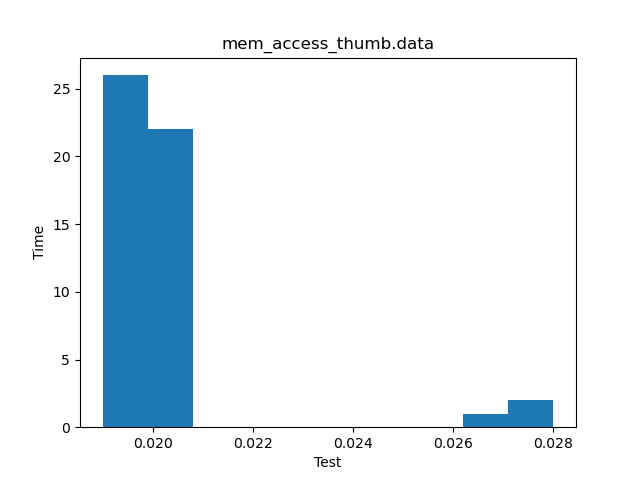
\includegraphics[width=\linewidth]{data/mem_access_thumb_histogram.png}
\end{figure}

\begin{figure}[H]
 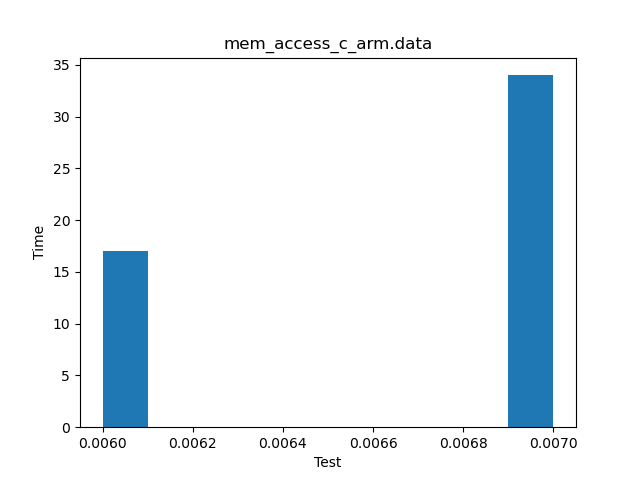
\includegraphics[width=\linewidth]{data/mem_access_c_arm_histogram.png}
\end{figure}

\begin{figure}[H]
 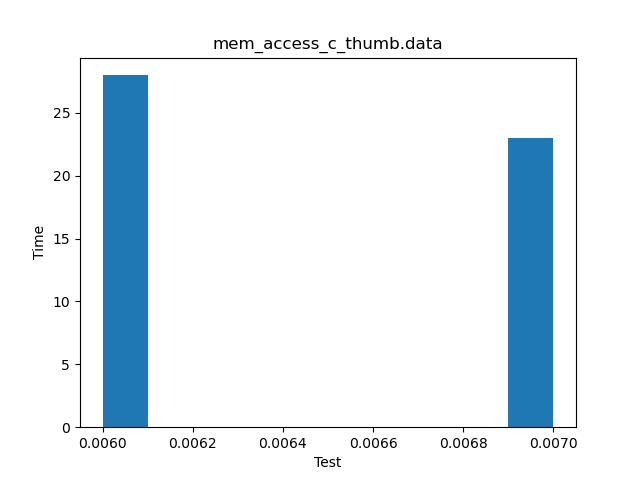
\includegraphics[width=\linewidth]{data/mem_access_c_thumb_histogram.png}
\end{figure}



\end{document}          
